% Generated from the Notion page by tools/notion2tex.py (see report/README.md).
\section{Introduction}\label{sec:1}

Single-image super-resolution (SR) reconstructs a high-resolution image from one low-resolution input \cite{ref1}. SRCNN \cite{ref2,ref3} was the first convolutional network to do this end to end and remains the simplest learned SR method: three convolutional layers applied to a bicubically upscaled image, trained to minimise the mean squared error against the high-resolution original. On the standard Set5 and Set14 benchmarks \cite{ref5,ref6} it improves the peak signal-to-noise ratio (PSNR) of the bicubic input by 1 to 3 dB depending on the image (Table~\ref{tab:13}).

\textbf{The algorithm.} Figure~\ref{fig:network} shows the network. The first layer extracts features with 64 kernels of 9$\times$9 on the single-channel input, the second maps them non-linearly with 32 kernels of 1$\times$1, and the third reconstructs one output channel with a 5$\times$5 kernel; the first two layers are followed by ReLU, the last is linear \cite{ref7}. Conv1 and Conv3 pad by edge replication so that the output has the same size as the input \cite{ref8}. The model is small, 8,129 parameters in all, but a single 255$\times$255 frame costs 522 million multiply-accumulate (MAC) operations, of which Conv1 alone is 64.5 \% (Table~\ref{tab:4}). This combination, a tiny parameter set and a large, perfectly regular arithmetic load with abundant data reuse between neighbouring pixels, is what makes a convolutional network a good match for an FPGA \cite{ref10}: the weights fit on chip, the computation can be unrolled across DSP slices, and the intermediate data never has to leave the device.

\begin{figure}[!htbp]
\centering
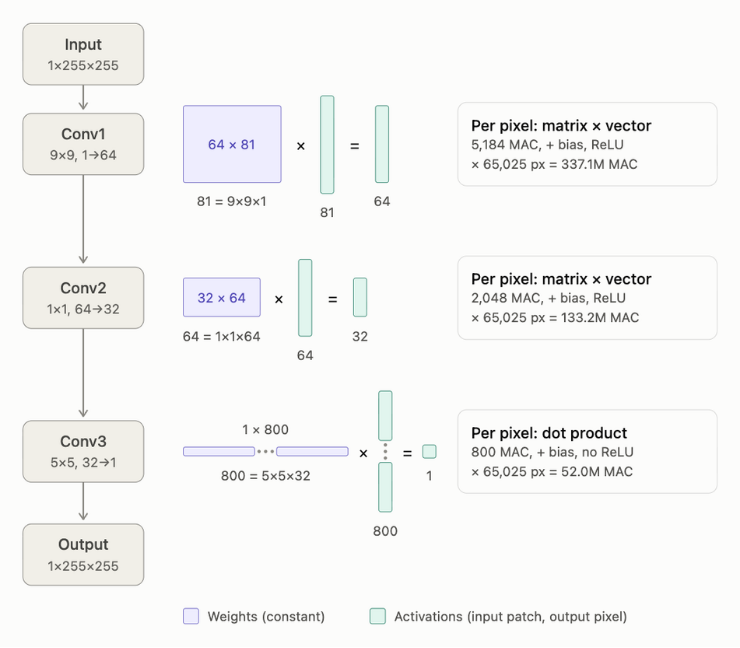
\includegraphics[width=0.78\figw]{figures/fig00-network.png}
\caption{The SRCNN network as implemented: Conv1 (9$\times$9, 1$\rightarrow$64 channels, ReLU), Conv2 (1$\times$1, 64$\rightarrow$32, ReLU) and Conv3 (5$\times$5, 32$\rightarrow$1, linear) on a 255$\times$255 single-channel input. Per output pixel each layer is a matrix--vector product with 5,184, 2,048 and 800 multiply-accumulates; over the 65,025 pixels of a frame that is 337.1 M, 133.2 M and 52.0 M, 522 million in all.}
\label{fig:network}
\end{figure}

\textbf{Platform and tool flow.} The target is the AMD Kria KV260 Vision AI Starter Kit \cite{ref11}, whose Zynq UltraScale+ MPSoC (device xck26-sfvc784-2LV-c) offers 1,248 DSP48E2 slices, 117,120 LUTs, 234,240 flip-flops, 5.1 Mb of block RAM and 18 Mb of UltraRAM in the programmable logic, next to a quad-core Arm processing system with DDR4. The accelerator is written in C++ and synthesised with Vitis HLS \cite{ref12}, integrated with the processing system in Vivado, and driven from Python through PYNQ \cite{ref13}.

\textbf{Goals.} Four goals were fixed at the start of the optimisation phase and are used as the specification against which Sections~\ref{sec:5} and \ref{sec:6} measure the result:

\begin{itemize}
\item \textbf{G1, function.} The accelerator keeps the original interface (the \texttt{srcnn} function with float arrays and parameters loaded from memory at run time), the 1-64-32-1 network and replicate padding. Its output must be bit-exact against a fixed-point reference on every one of the 13 Set14 images, and the mean PSNR of that reference on Set14 may be no more than 0.1 dB below the floating-point network.
\item \textbf{G2, speed.} The primary metric is milliseconds per 255$\times$255 frame, measured on the board. The goal is to make it as small as possible; no fixed target was set, because at the outset we had no basis for one beyond the baseline.
\item \textbf{G3, fit.} The design must place, route and meet timing on the xck26 device as an integrated PS+PL system.
\item \textbf{G4, evidence.} Every number reported must be traceable to an archived run, with its level of evidence stated: HLS estimate, RTL co-simulation, post-route implementation or on-board measurement.
\end{itemize}

\textbf{Approach.} The work has three stages. We first wrote a tiled, pipelined floating-point implementation of the original algorithm and verified it on the board (Section~\ref{sec:2}). It is correct and slow, and its profile shows why: the three layers run one after another, almost all DSP slices are idle, and all arithmetic is in single-precision float. Closing that gap is a search over a large space of HLS techniques, and each point in the space costs tens of minutes of synthesis and up to three hours of place-and-route to evaluate. Rather than search by hand, we handed the loop to general-purpose LLM coding agents (OpenAI Codex and Anthropic Claude Code) operating under a written experimental protocol: a fixed functional contract, one primary metric, explicit acceptance gates, an experiment card committed before every run, and an archive of every result including failures. We wrote the plans and reviewed the results; the agents wrote, ran and documented the experiments (Section~\ref{sec:3}). The design that emerged, a whole-network dataflow pipeline in 10-bit fixed point with Winograd convolution \cite{ref15,ref16} on Conv1 and two-products-per-DSP packing on Conv2, is explained decision by decision in Section~\ref{sec:4}. Finally, the IP was integrated, verified on the board and profiled, and the difference between its simulated and measured speed was traced to its causes (Section~\ref{sec:5}).

\textbf{Contributions.} The report makes three. First, a verified SRCNN accelerator whose on-board hardware time per frame falls from 2.238 s for the baseline to 2.938 ms, bit-exact against its fixed-point reference on every test image. Second, an auditable protocol for using general coding agents to search an HLS design space, with the finding that for this network the HLS logic estimates are pessimistic by about 2$\times$ and the clock estimates optimistic by about 2$\times$, so that a search ranked on HLS estimates would have chosen the wrong design. Third, a measured account of the gap between RTL simulation and the board, attributed with hardware counters to the clock configuration and to single-beat AXI reads on the input path.

The remainder of the report is organised as follows. Section~\ref{sec:2} analyses the algorithm and the baseline. Section~\ref{sec:3} describes the agent-driven exploration: the protocol, what it caught, and the decisions that shaped the search. Section~\ref{sec:4} explains the final architecture layer by layer. Section~\ref{sec:5} covers Vivado integration, on-board verification and performance debugging. Section~\ref{sec:6} discusses the results against the goals, the sources of the speedup, the method, and its limitations; Section~\ref{sec:7} concludes.
